%% nipping.tex -- NBS expansions relative to the must-expand floor |MVC|, with
%% and without HOG2's opposite-frontier discard (the -DADMISSIBLE rebuild).
%% One row per instance; 24 instances over 4 map/connectivity groups.
%% Values are exactly those of results/nbs_admissible_{test,batch2}.csv divided by
%% the mvc column of results/{cluster/combined_long,nbs_batch2_mvc}.csv.
%% Fragment: wrap in \begin{figure}...\caption{...}\end{figure}. Needs tikz+pgfplots.
\begingroup
\pgfplotsset{compat=1.16}
\definecolor{nipDefault}{RGB}{20,66,110}
\definecolor{nipAdm}{RGB}{176,74,16}
\tikzset{
  pairline/.style={line width=0.35pt, draw=gray!60},
  grpsep/.style={line width=0.25pt, draw=gray!45, densely dotted},
  grphead/.style={anchor=west, inner sep=0pt, font=\footnotesize},
}
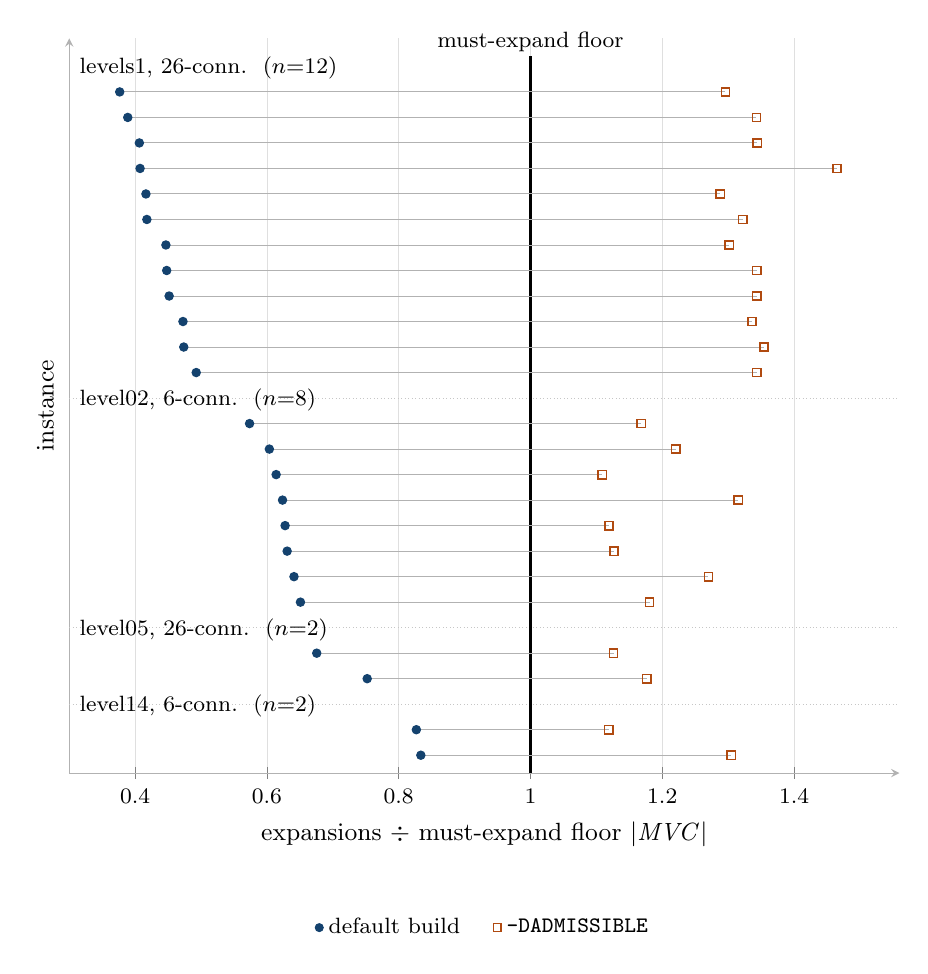
\begin{tikzpicture}
\begin{axis}[
  width=1.00\columnwidth, height=0.90\columnwidth,
  axis lines=left,
  axis line style={line width=0.35pt, draw=gray!60},
  xmin=0.30, xmax=1.56,
  ymin=0.3, ymax=29.1,
  enlargelimits=false,
  clip=false,
  xtick={0.4,0.6,0.8,1.0,1.2,1.4},
  xticklabel style={/pgf/number format/fixed, /pgf/number format/precision=1},
  ytick=\empty,
  tick label style={font=\footnotesize},
  label style={font=\small},
  xlabel={expansions $\div$ must-expand floor $|\mathit{MVC}|$},
  ylabel={instance},
  xmajorgrids=true,
  grid style={line width=0.2pt, draw=gray!25},
  legend style={font=\footnotesize, at={(0.5,-0.185)}, anchor=north,
                legend columns=2, draw=none, fill=none, inner sep=1pt,
                /tikz/every even column/.append style={column sep=10pt}},
  legend cell align=left,
  legend image post style={scale=0.95},
]
%% group separators and headers
\draw[grpsep] (axis cs:0.30,15) -- (axis cs:1.56,15);
\draw[grpsep] (axis cs:0.30,6) -- (axis cs:1.56,6);
\draw[grpsep] (axis cs:0.30,3) -- (axis cs:1.56,3);
\node[grphead] at (axis cs:0.315,27.92) {levels1, 26-conn.\ \ ($n{=}12$)};
\node[grphead] at (axis cs:0.315,14.92) {level02, 6-conn.\ \ ($n{=}8$)};
\node[grphead] at (axis cs:0.315,5.92) {level05, 26-conn.\ \ ($n{=}2$)};
\node[grphead] at (axis cs:0.315,2.92) {level14, 6-conn.\ \ ($n{=}2$)};
%% the must-expand floor: expansions = |MVC|
\draw[line width=0.9pt, draw=black] (axis cs:1,0.3) -- (axis cs:1,28.4);
\node[anchor=south, inner sep=1.5pt, font=\footnotesize] at (axis cs:1,28.4)
  {must-expand floor};
%% one thin connector per instance
\draw[pairline] (axis cs:0.3766,27) -- (axis cs:1.2959,27);
\draw[pairline] (axis cs:0.3888,26) -- (axis cs:1.3430,26);
\draw[pairline] (axis cs:0.4064,25) -- (axis cs:1.3443,25);
\draw[pairline] (axis cs:0.4075,24) -- (axis cs:1.4651,24);
\draw[pairline] (axis cs:0.4164,23) -- (axis cs:1.2881,23);
\draw[pairline] (axis cs:0.4178,22) -- (axis cs:1.3222,22);
\draw[pairline] (axis cs:0.4467,21) -- (axis cs:1.3018,21);
\draw[pairline] (axis cs:0.4479,20) -- (axis cs:1.3435,20);
\draw[pairline] (axis cs:0.4516,19) -- (axis cs:1.3436,19);
\draw[pairline] (axis cs:0.4726,18) -- (axis cs:1.3363,18);
\draw[pairline] (axis cs:0.4738,17) -- (axis cs:1.3545,17);
\draw[pairline] (axis cs:0.4927,16) -- (axis cs:1.3432,16);
\draw[pairline] (axis cs:0.5737,14) -- (axis cs:1.1680,14);
\draw[pairline] (axis cs:0.6037,13) -- (axis cs:1.2204,13);
\draw[pairline] (axis cs:0.6140,12) -- (axis cs:1.1088,12);
\draw[pairline] (axis cs:0.6237,11) -- (axis cs:1.3155,11);
\draw[pairline] (axis cs:0.6276,10) -- (axis cs:1.1192,10);
\draw[pairline] (axis cs:0.6307,9) -- (axis cs:1.1266,9);
\draw[pairline] (axis cs:0.6411,8) -- (axis cs:1.2701,8);
\draw[pairline] (axis cs:0.6509,7) -- (axis cs:1.1807,7);
\draw[pairline] (axis cs:0.6756,5) -- (axis cs:1.1261,5);
\draw[pairline] (axis cs:0.7522,4) -- (axis cs:1.1763,4);
\draw[pairline] (axis cs:0.8268,2) -- (axis cs:1.1189,2);
\draw[pairline] (axis cs:0.8336,1) -- (axis cs:1.3045,1);
\addplot[only marks, mark=*, mark size=1.5pt, draw=nipDefault, fill=nipDefault]
  coordinates {
      (0.3766,27) (0.3888,26) (0.4064,25) (0.4075,24) (0.4164,23) (0.4178,22)
      (0.4467,21) (0.4479,20) (0.4516,19) (0.4726,18) (0.4738,17) (0.4927,16)
      (0.5737,14) (0.6037,13) (0.6140,12) (0.6237,11) (0.6276,10) (0.6307,9)
      (0.6411,8) (0.6509,7) (0.6756,5) (0.7522,4) (0.8268,2) (0.8336,1)
  };
\addlegendentry{default build}
\addplot[only marks, mark=square, mark size=1.5pt, line width=0.55pt, draw=nipAdm]
  coordinates {
      (1.2959,27) (1.3430,26) (1.3443,25) (1.4651,24) (1.2881,23) (1.3222,22)
      (1.3018,21) (1.3435,20) (1.3436,19) (1.3363,18) (1.3545,17) (1.3432,16)
      (1.1680,14) (1.2204,13) (1.1088,12) (1.3155,11) (1.1192,10) (1.1266,9)
      (1.2701,8) (1.1807,7) (1.1261,5) (1.1763,4) (1.1189,2) (1.3045,1)
  };
\addlegendentry{\texttt{-DADMISSIBLE}}
\end{axis}
\end{tikzpicture}
\endgroup
